% example-4-summary.tex
% Self-contained extract from example.tex (compile: pdflatex example-4-summary.tex, run twice).

\documentclass[11pt]{article}

\usepackage[margin=1in]{geometry}
\usepackage{amsmath}
\usepackage{enumitem}
\usepackage{xcolor}
\usepackage{soul}
\usepackage{tikz}
\usetikzlibrary{arrows.meta,positioning,calc,backgrounds}

% --- atomic-unit highlight roles ---
\definecolor{cId}   {RGB}{210,228,248}   % neutral / uncontested atom
\definecolor{cEarly}{RGB}{198,231,201}    % reliable atom (from source A)
\definecolor{cLate} {RGB}{248,205,205}    % false atom (from source B)

% \fu{colour}{span}{label}: highlight a clause and tag it with its atomic-unit id.
% \hl (soul) wraps across line breaks.
\sethlcolor{cId}
\newcommand{\fu}[3]{{\sethlcolor{#1}\hl{#2}}\,\textsuperscript{\textbf{\scriptsize #3}}}

\title{Example 4: Reliable vs.\ Unreliable Source Summary}
\author{FactReasoner --- Ideation}
\date{\today}

\begin{document}
\maketitle
\section{Synthesizing a summary from a reliable and an unreliable source}

This example starts from two source paragraphs about the same subject. Source
\textbf{A} is largely accurate; source \textbf{B} is a sensational news piece
containing several factual errors that \emph{contradict} A. We then synthesize a
summary \textbf{S} that deliberately interleaves claims from both, so that S
contains both logical-implication chains and positional invalidations, and we
analyse S with the usual decomposition.

\subsection*{Source A (reliable)}
\begin{quote}\small
Keyara Jones is an American college basketball player who played in the NCAA
Division I women's basketball league. Jones played college basketball for the
University of Alabama during the 2020--2021 season, as a member of the Crimson
Tide women's basketball team, which competes in the Southeastern Conference (SEC)
of NCAA Division I. The NCAA Division I women's basketball league consists of 356
teams and is considered the highest level of women's college basketball in the
United States. According to the University of Alabama's athletic website, Jones
is listed as a \emph{guard from Birmingham, Alabama}, and was a member of the
women's basketball team during the 2020--2021 season; ESPN and CBS Sports also
reported on her performances that season.
\end{quote}

\subsection*{Source B (unreliable --- contains factual errors)}
\begin{quote}\small
``Breaking News: Alabama's Keyara Jones Makes History as First Female Player in
NCAA Division~I \emph{Men's} Basketball.'' The 20-year-old junior, a 5$'$10$''$
\emph{guard from Montgomery, Alabama}, made her debut last night. Averaging 18
points and 7 rebounds per game, she led the Alabama women's team to a Sweet~16
appearance last season. Coach Nate Oats praised her, and a sports sociologist
called it a milestone for gender equality. ``According to NCAA data, only 12\% of
Division~I men's basketball players are women,'' the piece reports, framing
Jones' entry as a step toward greater gender representation; several NBA teams
are said to be scouting her.
\end{quote}

\noindent
\textbf{Errors in B (each contradicts A).} (i)~Jones joined an NCAA Division~I
\emph{men's} team --- A has her on the \emph{women's} team. (ii)~She is a guard
from \emph{Montgomery} --- A's cited source says \emph{Birmingham}.
(iii)~The ``12\% of men's players are women'' statistic is internally absurd.
The fabricated junior/height/Sweet~16/NBA-scouting details have no support in A.

\subsection*{Synthesized summary S}

S is written to interleave B's sensational (false) framing \emph{first} with A's
reliable record \emph{afterward}, so that the later (true) atoms positionally
invalidate the earlier (false) ones, while several implication chains run within
each block.

\noindent\textbf{Plain text.}
\begin{quote}
Keyara Jones is an American college basketball player from Montgomery, Alabama,
who plays guard for the University of Alabama. During the 2020--2021 season she
made history as the first woman to join an NCAA Division~I men's basketball team,
averaging 18 points per game and leading Alabama to a Sweet~16 appearance.
Because she competed in the men's league, her achievement was hailed as a
milestone for gender equality, and NCAA data showing that 12\% of Division~I
men's players are women was cited to underscore the trend. In fact, the
University of Alabama's athletic website lists Jones as a guard from Birmingham,
Alabama, who was a member of the women's basketball team during the 2020--2021
season. The Crimson Tide women's team competes in the Southeastern Conference of
NCAA Division~I women's basketball, which is the highest level of women's college
basketball in the United States and consists of 356 teams.
\end{quote}

\noindent\textbf{Annotated.} Each clause is one atomic unit
\textsuperscript{\textbf{\scriptsize S\textit{n}}}. Red marks a false atom
imported from source~B, green a reliable atom from source~A; neutral (blue) atoms
are uncontested.

\begin{quote}
\fu{cId}{Keyara Jones is an American college basketball player}{S1}
\fu{cLate}{from Montgomery, Alabama}{S2},
\fu{cId}{who plays guard for the University of Alabama}{S3}. During the
2020--2021 season she
\fu{cLate}{made history as the first woman to join an NCAA Division~I men's basketball team}{S4},
\fu{cId}{averaging 18 points per game}{S5} and
\fu{cId}{leading Alabama to a Sweet~16 appearance}{S6}. Because she
\fu{cLate}{competed in the men's league}{S7},
\fu{cLate}{her achievement was hailed as a milestone for gender equality}{S8}, and
\fu{cLate}{NCAA data showing that 12\% of Division~I men's players are women}{S9}
\fu{cLate}{was cited to underscore the trend}{S10}. In fact, the
\fu{cEarly}{University of Alabama's athletic website lists Jones as a guard from Birmingham, Alabama}{S11},
\fu{cEarly}{who was a member of the women's basketball team during the 2020--2021 season}{S12}.
\fu{cEarly}{The Crimson Tide women's team competes in the Southeastern Conference of NCAA Division~I women's basketball}{S13},
\fu{cEarly}{which is the highest level of women's college basketball in the United States}{S14} and
\fu{cEarly}{consists of 356 teams}{S15}.
\end{quote}

\subsection*{Atomic units of S (self-contained, in order of appearance)}
\begin{enumerate}[label=\textbf{S\arabic*.},leftmargin=*]
  \item Keyara Jones is an American college basketball player.
  \item Keyara Jones is from Montgomery, Alabama.
  \item Keyara Jones plays guard for the University of Alabama.
  \item During the 2020--2021 season Keyara Jones made history as the first woman to join an NCAA Division~I men's basketball team.
  \item Keyara Jones averaged 18 points per game.
  \item Keyara Jones led Alabama to a Sweet~16 appearance.
  \item Keyara Jones competed in the men's basketball league.
  \item Keyara Jones' achievement was hailed as a milestone for gender equality.
  \item NCAA data show that 12\% of Division~I men's basketball players are women.
  \item The 12\% statistic was cited to underscore the gender-equality trend.
  \item The University of Alabama's athletic website lists Keyara Jones as a guard from Birmingham, Alabama.
  \item Keyara Jones was a member of the University of Alabama women's basketball team during the 2020--2021 season.
  \item The Crimson Tide women's team competes in the Southeastern Conference of NCAA Division~I women's basketball.
  \item NCAA Division~I women's basketball is the highest level of women's college basketball in the United States.
  \item NCAA Division~I women's basketball consists of 356 teams.
\end{enumerate}

\subsection*{Relations}

\textbf{Logical prerequisites ($A \rightarrow B$).}
\begin{itemize}[leftmargin=*]
  \item S3 $\rightarrow$ S4 --- playing for Alabama is presupposed by joining an Alabama (men's) team.
  \item S4 $\rightarrow$ S7 --- joining a men's team is what it means to compete in the men's league.
  \item S7 $\rightarrow$ S8 --- competing in the men's league is the stated ground for the gender-equality acclaim.
  \item S9 $\rightarrow$ S10 --- the 12\% statistic is what is cited to underscore the trend.
  \item S8,\,S10 share the gender-equality framing (S10 reinforces S8).
  \item S12 $\rightarrow$ S13 --- membership of the women's team is presupposed by that team competing in the SEC.
  \item S13 $\rightarrow$ S14 --- the women's league existing/being top-level is presupposed by S13 placing the team in it.
  \item S14 $\rightarrow$ S15 --- the league being characterised (top level) is presupposed by counting its 356 teams.
  \item S1 $\rightarrow$ S3 --- being a college basketball player is presupposed by playing guard for a specific program.
\end{itemize}

\noindent
\textbf{Position invalidations ($A \neq B$).} The reliable atoms S11 and S12
(from source A), appearing \emph{after} B's framing, positionally invalidate the
earlier false atoms.

\begin{itemize}[leftmargin=*]
  \item S11 $\neq$ S2 --- the cited website says \emph{Birmingham}, contradicting ``from Montgomery.''
  \item S12 $\neq$ S4 --- being on the \emph{women's} team contradicts ``first woman on a men's team.''
  \item S12 $\neq$ S7 --- women's-team membership contradicts ``competed in the men's league.''
  \item S12 $\neq$ S8 --- with no men's-league entry, the gender-equality milestone collapses.
  \item S12 $\neq$ S10 --- the men's-representation framing is voided once the men's-league premise fails.
  \item S9 $\neq$ S9 (self-inconsistent) --- ``12\% of \emph{men's} players are women'' is internally contradictory regardless of position.
\end{itemize}

\noindent
\textbf{Note.} The Sweet~16 and 18-ppg atoms (S5, S6) are unsupported by A but
not directly contradicted by it; they are left as neither implied nor
invalidated. The contradiction structure is concentrated on S12 (true
women's-team membership) overturning the men's-league thread S4--S10.

\subsection*{Relation graph}

Solid blue arrows are logical prerequisites ($A \rightarrow B$); dashed red
arrows are position invalidations ($A \neq B$). False atoms imported from B are
tinted red; the two reliable invalidating atoms from A (S11, S12) are green and
highlighted. The self-contradictory statistic S9 carries a red self-loop.

\begin{center}
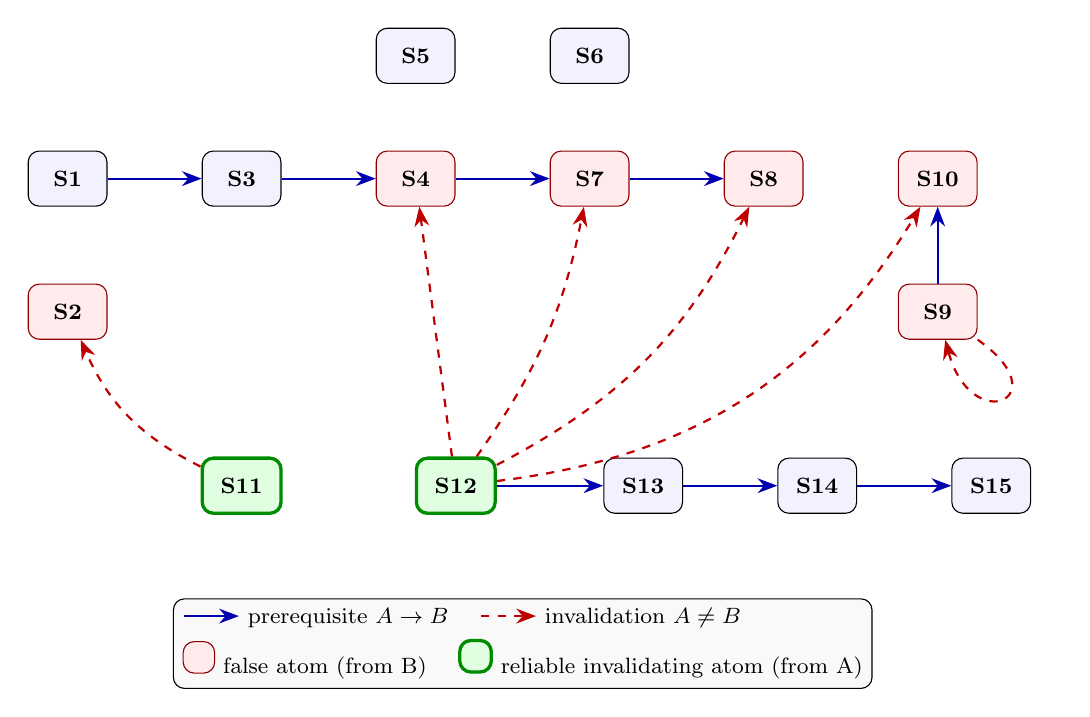
\begin{tikzpicture}[
    >={Stealth[length=2.5mm]},
    x=17mm, y=13mm,
    snode/.style={draw,rounded corners,minimum width=10mm,minimum height=7mm,
                  inner sep=1pt,font=\footnotesize\bfseries,fill=blue!5},
    falsey/.style={snode,fill=red!8,draw=red!55!black},
    truthy/.style={snode,fill=green!12,draw=green!55!black,very thick},
    prereq/.style={->,blue!70!black,thick},
    invalid/.style={->,red!75!black,dashed,thick},
  ]

  % --- top: B's false "men's league" thread (left to right) ---
  \node[snode]  (s1) at (0,3)   {S1};
  \node[falsey] (s2) at (0,1.7) {S2};
  \node[snode]  (s3) at (1.3,3) {S3};
  \node[falsey] (s4) at (2.6,3) {S4};
  \node[falsey] (s7) at (3.9,3) {S7};
  \node[falsey] (s8) at (5.2,3) {S8};
  \node[falsey] (s10) at (6.5,3) {S10};
  \node[falsey] (s9)  at (6.5,1.7) {S9};

  % --- unsupported (neither) ---
  \node[snode]  (s5) at (2.6,4.2) {S5};
  \node[snode]  (s6) at (3.9,4.2) {S6};

  % --- bottom: A's reliable thread ---
  \node[truthy] (s11) at (1.3,0)  {S11};
  \node[truthy] (s12) at (2.9,0)  {S12};
  \node[snode]  (s13) at (4.3,0)  {S13};
  \node[snode]  (s14) at (5.6,0)  {S14};
  \node[snode]  (s15) at (6.9,0)  {S15};

  % --- prerequisite edges ---
  \draw[prereq] (s1) -- (s3);
  \draw[prereq] (s3) -- (s4);
  \draw[prereq] (s4) -- (s7);
  \draw[prereq] (s7) -- (s8);
  \draw[prereq] (s9) -- (s10);
  \draw[prereq] (s12) -- (s13);
  \draw[prereq] (s13) -- (s14);
  \draw[prereq] (s14) -- (s15);

  % --- invalidation edges from the reliable atoms ---
  \draw[invalid] (s11) to[bend left=20] (s2);
  \draw[invalid] (s12) -- (s4);
  \draw[invalid] (s12) to[bend right=12] (s7);
  \draw[invalid] (s12) to[bend right=18] (s8);
  \draw[invalid] (s12) to[bend right=26] (s10);

  % --- self-contradiction loop on S9 ---
  \draw[invalid] (s9) to[out=-35,in=-75,looseness=8] (s9);

  % --- legend ---
  \node[draw,fill=gray!5,rounded corners,anchor=north,align=left,
        font=\footnotesize] at (3.4,-1.1) {
    \tikz\draw[prereq](0,0)--(7mm,0);~prerequisite $A\rightarrow B$
    \quad
    \tikz\draw[invalid](0,0)--(7mm,0);~invalidation $A\neq B$\\[3pt]
    \tikz\node[falsey,minimum width=4mm,minimum height=4mm]{};~false atom (from B)
    \quad
    \tikz\node[truthy,minimum width=4mm,minimum height=4mm]{};~reliable invalidating atom (from A)
  };

\end{tikzpicture}
\end{center}

\noindent\emph{(S5 and S6 --- the unsupported 18-ppg and Sweet~16 claims --- are
shown without relation edges: A neither implies nor contradicts them.)}

\end{document}
